\chapter{Acoustic Ray Tracing Simulator (ARTS)}\label{chap:experiments}
In this chapter the implementation of the presented methods in \chapref{chap:approach} will be introduced and how ARTS can be used for a simple LOS (line of sight) localization algorithm using multilateration.
Furthermore the run times of the mentioned modules "Ray Tracer" and "Path Sampler" in the previous chapter will be presented and discussed.\newline
The source code for ARTS can be found on \url{https://github.com/mguc/arts}.
Use the README to get started.
All the references made in this chapter are based on \textbf{v1.0.0} of ARTS and a tag with that version can be found on the repository.

All tests have been performed on a system with an Intel Core i9-8950HK CPU @ 2.90GHz.

\newpage
\section{Setup Data}
There were mainly three environments used for testing:

1. A room called "reference room" which features a cuboid representing a 4m x 5m x 3m room. The origin $(0,0,0)$ is located in the center of the room.
\begin{figure}[H]
    \begin{center}
    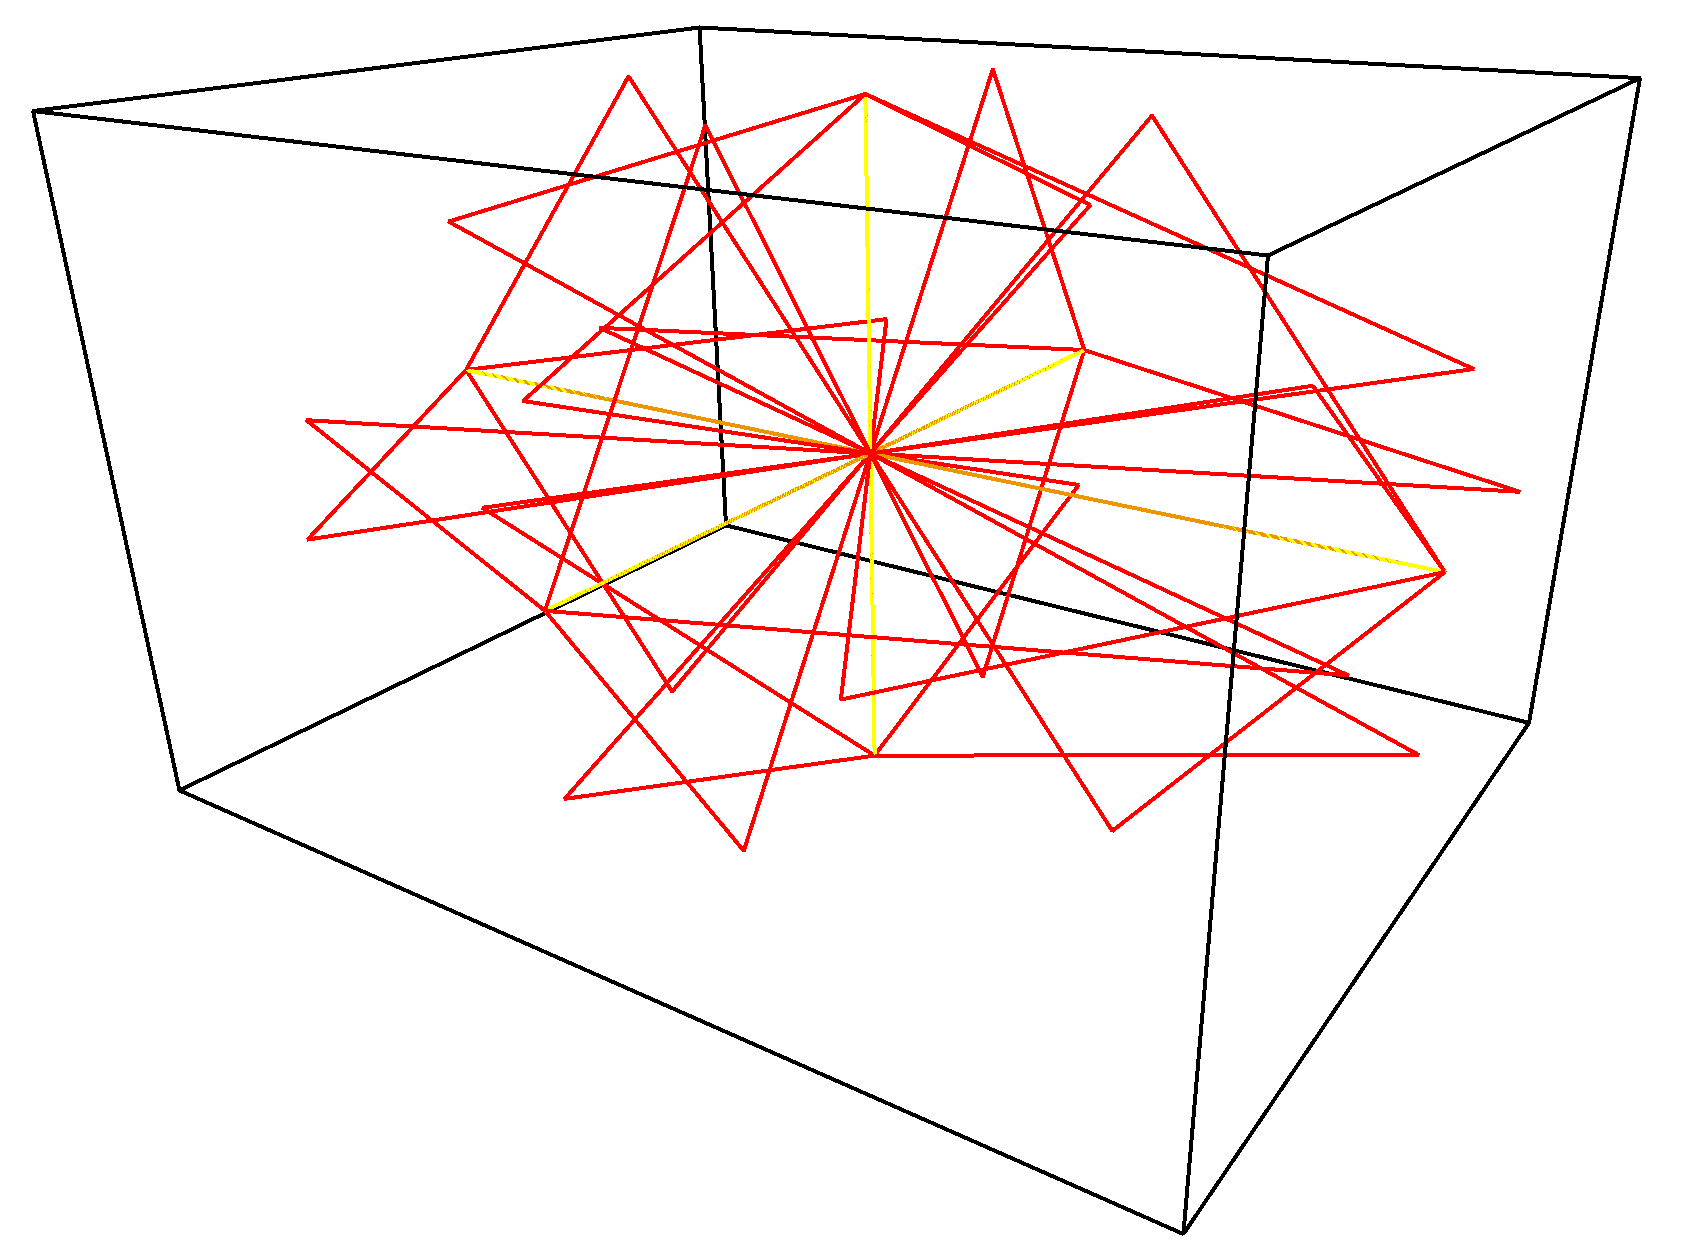
\includegraphics[width=\textwidth]{figures/experiments/reference_room.png}
    \end{center}
    \caption[Reference Room 4m x 5m x 3m]{Reference Room 4m x 5m x 3m}
    \label{fig:referenceRoom}
\end{figure}

\newpage
2. The "Tube", which only contains a "floor" and a "ceiling". Floor and ceiling are 1m apart and have a surface area of 2m x 2m. It looks like a tube in $x$-$z$ or $y$-$z$ view, therefore the name.
\begin{figure}[H]
    \begin{center}
    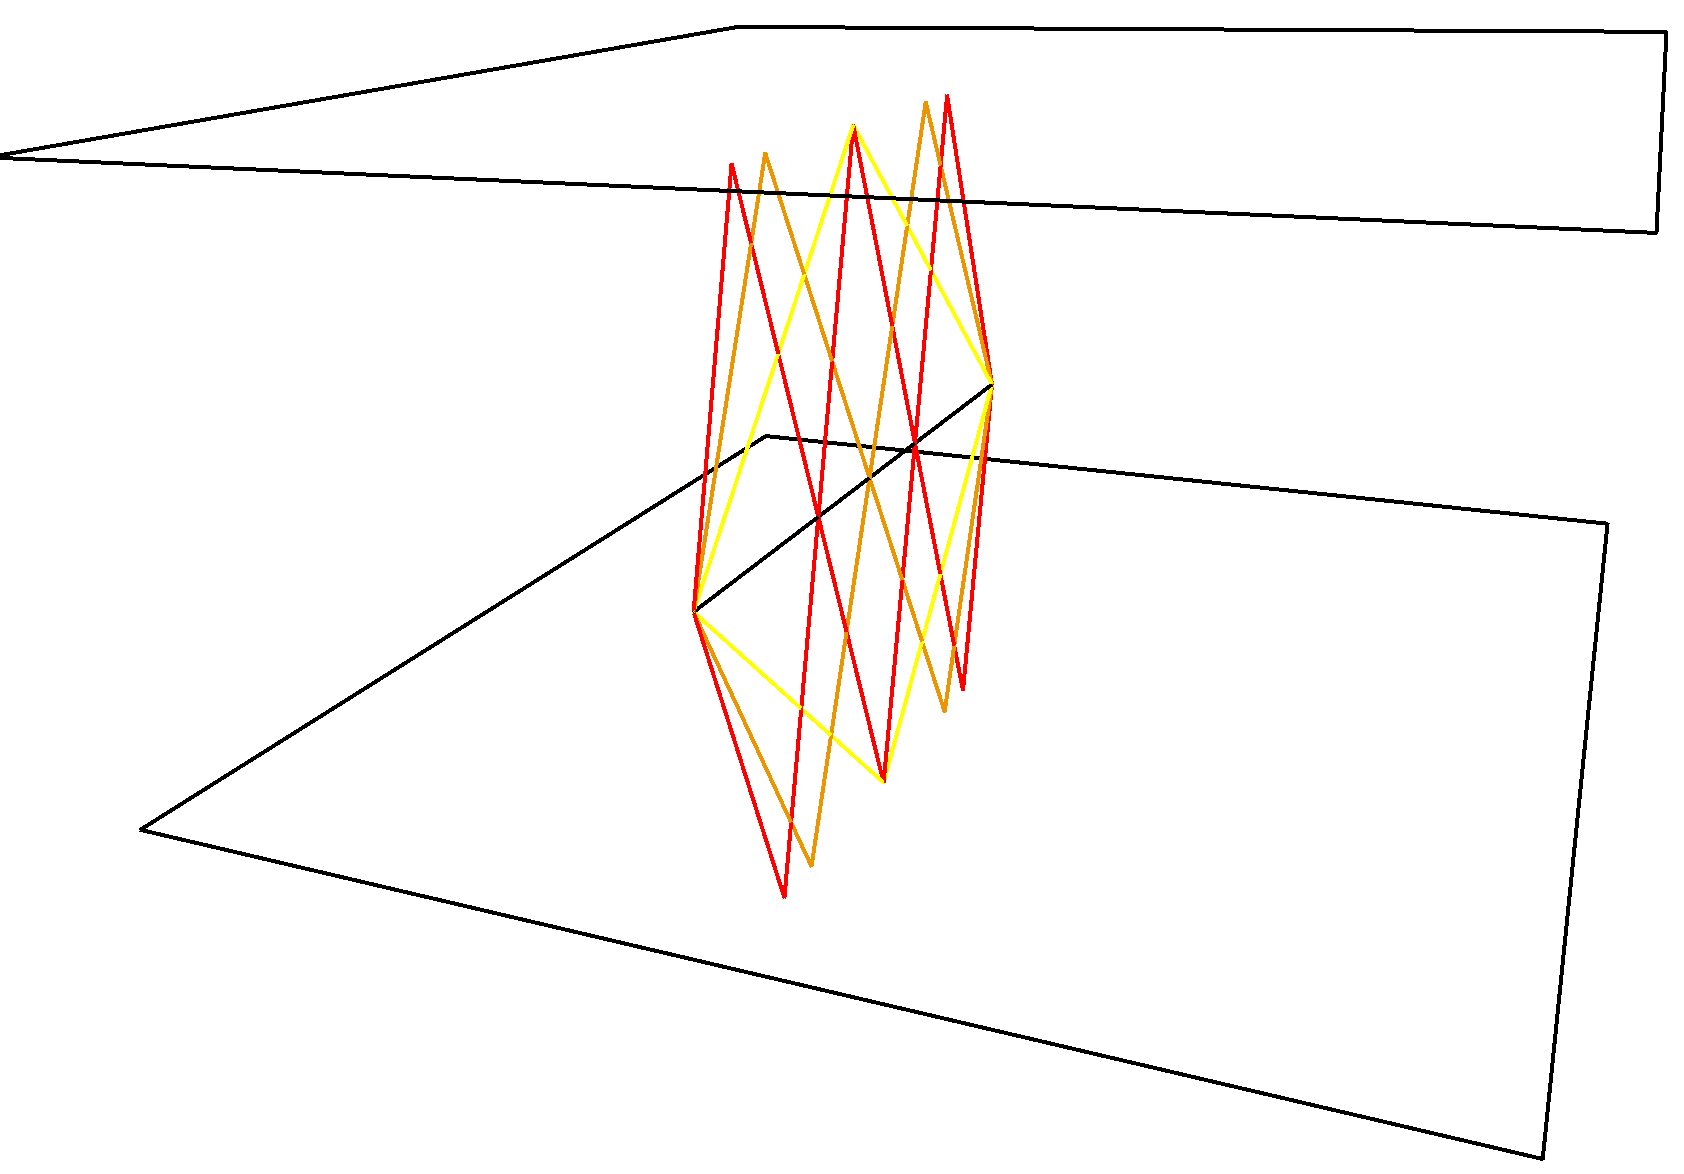
\includegraphics[width=\textwidth]{figures/experiments/tube_100.png}
    \end{center}
    \caption[Tube with Source at $(1,0,0)$ and Receiver at $(0,0,0)$]{Tube with Source at $(1,0,0)$ and Receiver at $(0,0,0)$}
    \label{fig:tube}
\end{figure}

\newpage
"Matryoshka Cube" which consists of $X$ nested cubes representing an environment with $6X$ obstacles $Q_1 ... Q_{6X}$.
\begin{figure}[H]
    \begin{center}
    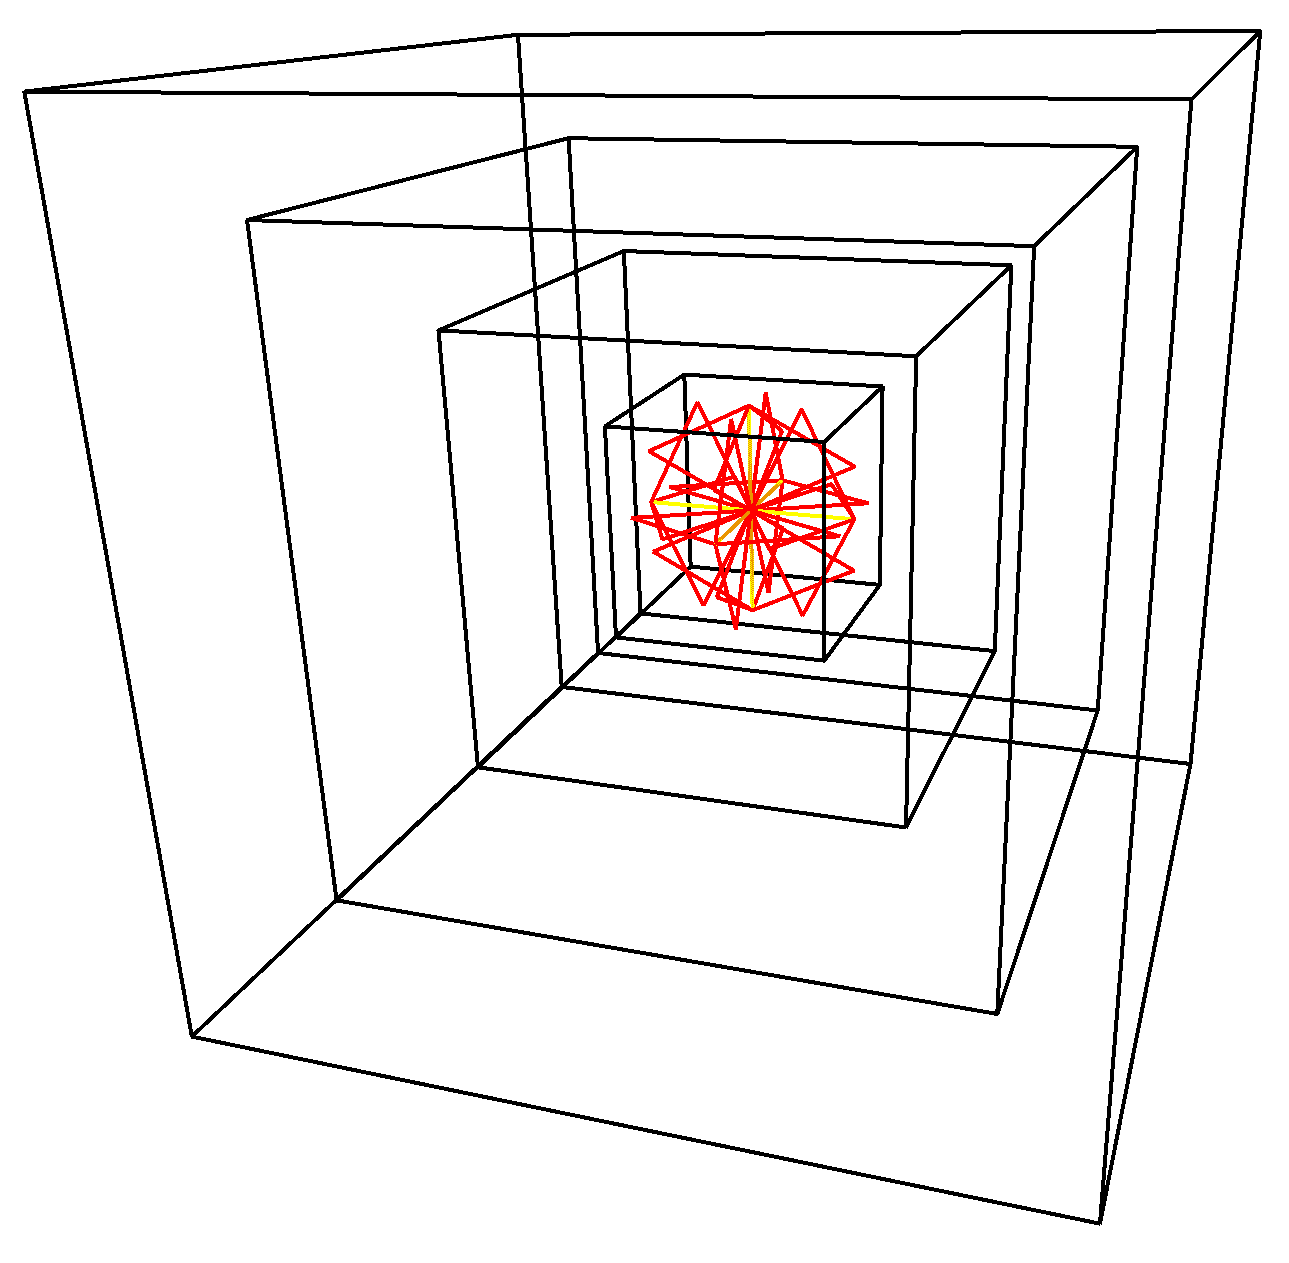
\includegraphics[width=\textwidth]{figures/experiments/matryoshka_4.png}
    \end{center}
    \caption[Matryoshka Cube with $X=4$ nested cubes]{Matryoshka Cube with $X=4$ nested cubes}
    \label{fig:matryoshka4}
\end{figure}


\newpage
\section{Model Simplification}\label{sec:modelSimplification}
In \textbf{v1.0.0} of ARTS not all features and properties discussed in the previous \chapref{chap:approach} have been implemented.\newline
Obstacles $Q_k$ will be treated as "perfect" reflectors, resulting in a reflection coefficient $\gamma_k = 1$ for all $k \in \{1,...,K\}$.
Receivers and Sources will use a rectangular FOV function resulting in $f_{FOV}(\theta_r, \varphi_r) = 1$ and $g_{FOV}(\theta_s, \varphi_s) = 1$.
This simplifies \eqref{eq:receiver} and results in the following receiver sampling equation:
\begin{equation}
    r_{ij}[n] = \sum_{P \in G_{ij}} \mathcal{L}(d_P) \cdot x_s(n \cdot T_r - \frac{d_P}{c_{\text{air}}})
\end{equation}
For $x_s(t)$ a slightly modified unit sample function $\delta[n]$ will be used, see \figref{fig:delta}.
The width of the pulse will be extended to match the sampling width $T_r$ of the receivers.
The pulse width of $\delta[n]$ will be extended such that $T_p < T_r$.
This will ensure that the pulse is seen by the receiver exactly once.
The sampling frequency for the receivers is set to 1MHz therefore resulting in a sampling width of $T_r = 10^{-6}\text{s}$.
\begin{figure}[H]
    \begin{center}
    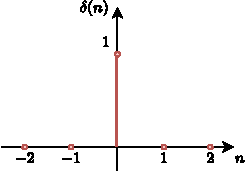
\includegraphics[width=0.5\textwidth]{figures/experiments/figDelta.pdf}
    \end{center}
    \caption[Unit sample function $\delta(n)$]{Unit sample function $\delta(n)$}
    \label{fig:delta}
\end{figure}

One big advantage of this approach is that the "room impulse response" (RIR) for a source location can be obtained.
The RIR will represent the travel time for the existing paths $P \in G_{ij}$.
This also means that a potential signal pre-processing can be skipped for estimators. In \figref{fig:RIR} the RIR for the reference room can be seen for a receiver and source sitting at the same location $(0,0,0)$.
\begin{figure}[H]
    \begin{center}
    \subfloat[RIR for $L=1$]{
        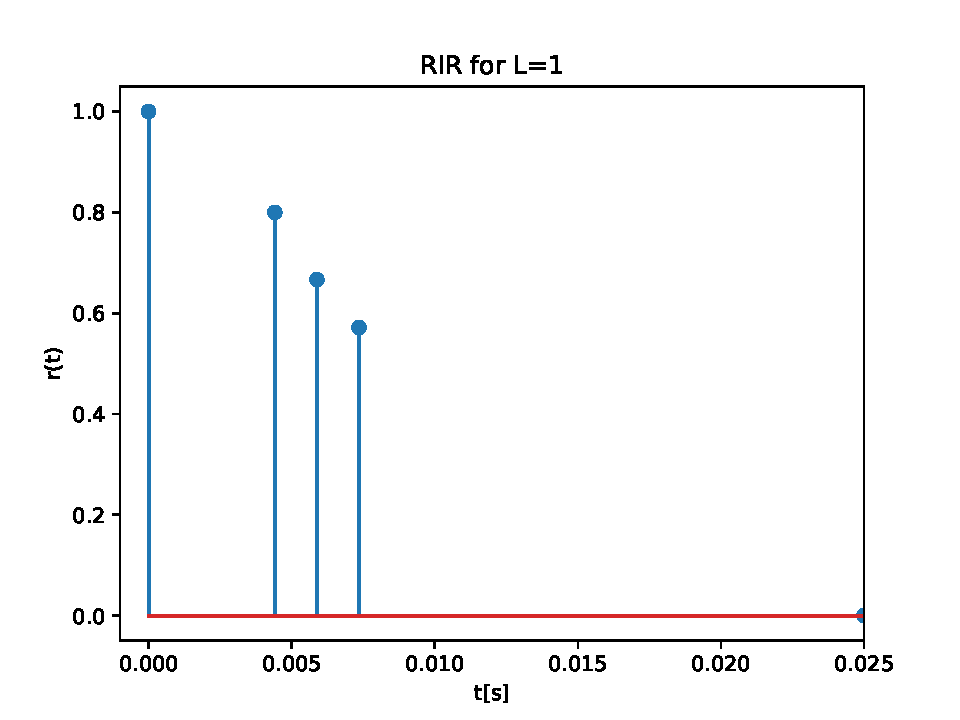
\includegraphics[width=\textwidth/2]{figures/experiments/rir1.pdf}
    }
    \subfloat[RIR for $L=2$]{
        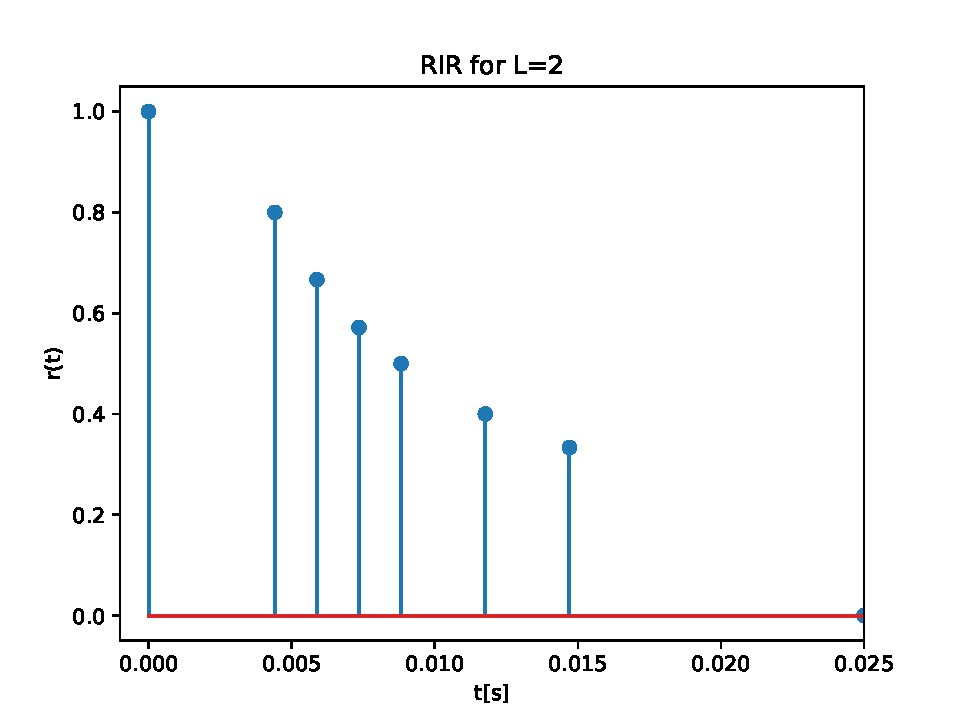
\includegraphics[width=\textwidth/2]{figures/experiments/rir2.pdf}
    }\\
    \subfloat[RIR for $L=3$]{
        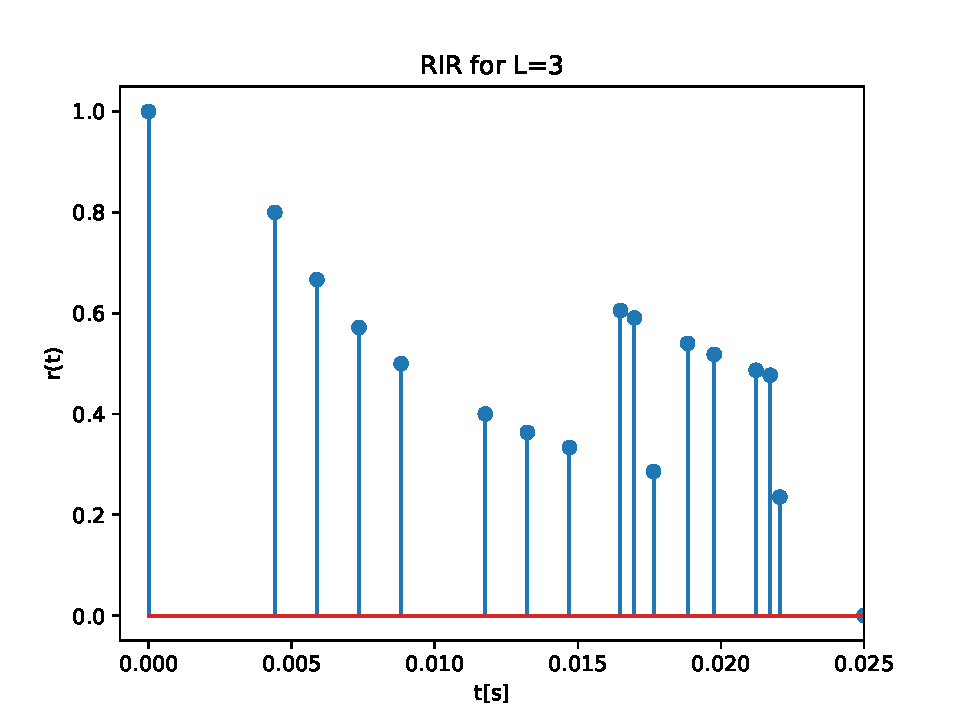
\includegraphics[width=\textwidth]{figures/experiments/rir3.pdf}
    }
    \end{center}
    \caption[Reference Room RIR]{Reference Room RIR}
    \label{fig:RIR}
\end{figure}


\section{ARTS Input Data}
In the ARTS repository the input data is located in the resource folder "rsc" and split by type: environment, receiver and source.

\textbf{Obstacles $Q_k$}\newline
The "Wavefront .obj file" format \cite{mreddy} will be used to represent the environment geometry and its obstacles $Q_k$. 
It is a format which is human readable and easy to comprehend. 
Most 3D modelling tools support the OBJ format and therefore make it a suitable candidate to define rooms and obstacles. 
This is a snippet for the reference room exported from Blender \cite{blender}:
\begin{verbatim}
    # Blender v2.79 (sub 0) OBJ File: '4x5x3room.blend'
    # www.blender.org
    mtllib 4x5x3room.mtl
    o Cube
    v 2.0 2.5 -1.5
    v 2.0 -2.5 -1.5
    v -2.0 -2.5 -1.5
    v -2.0 2.5 -1.5
    v 2.0 2.5 1.5
    v 2.0 -2.5 1.5
    v -2.0 -2.5 1.5
    v -2.0 2.5 1.5
    ...
    f 1//1 2//1 3//1 4//1
    f 5//2 8//2 7//2 6//2
    f 1//3 5//3 6//3 2//3
    f 2//4 6//4 7//4 3//4
    f 3//5 7//5 8//5 4//5
    f 5//6 1//6 4//6 8//6
\end{verbatim}

A line with a "v" represents a vertex (point in 3D) and "f" defines a face with vertex indices.
In \figref{fig:house} a more advanced 3D model is shown.
\begin{figure}[H]
    \begin{center}
    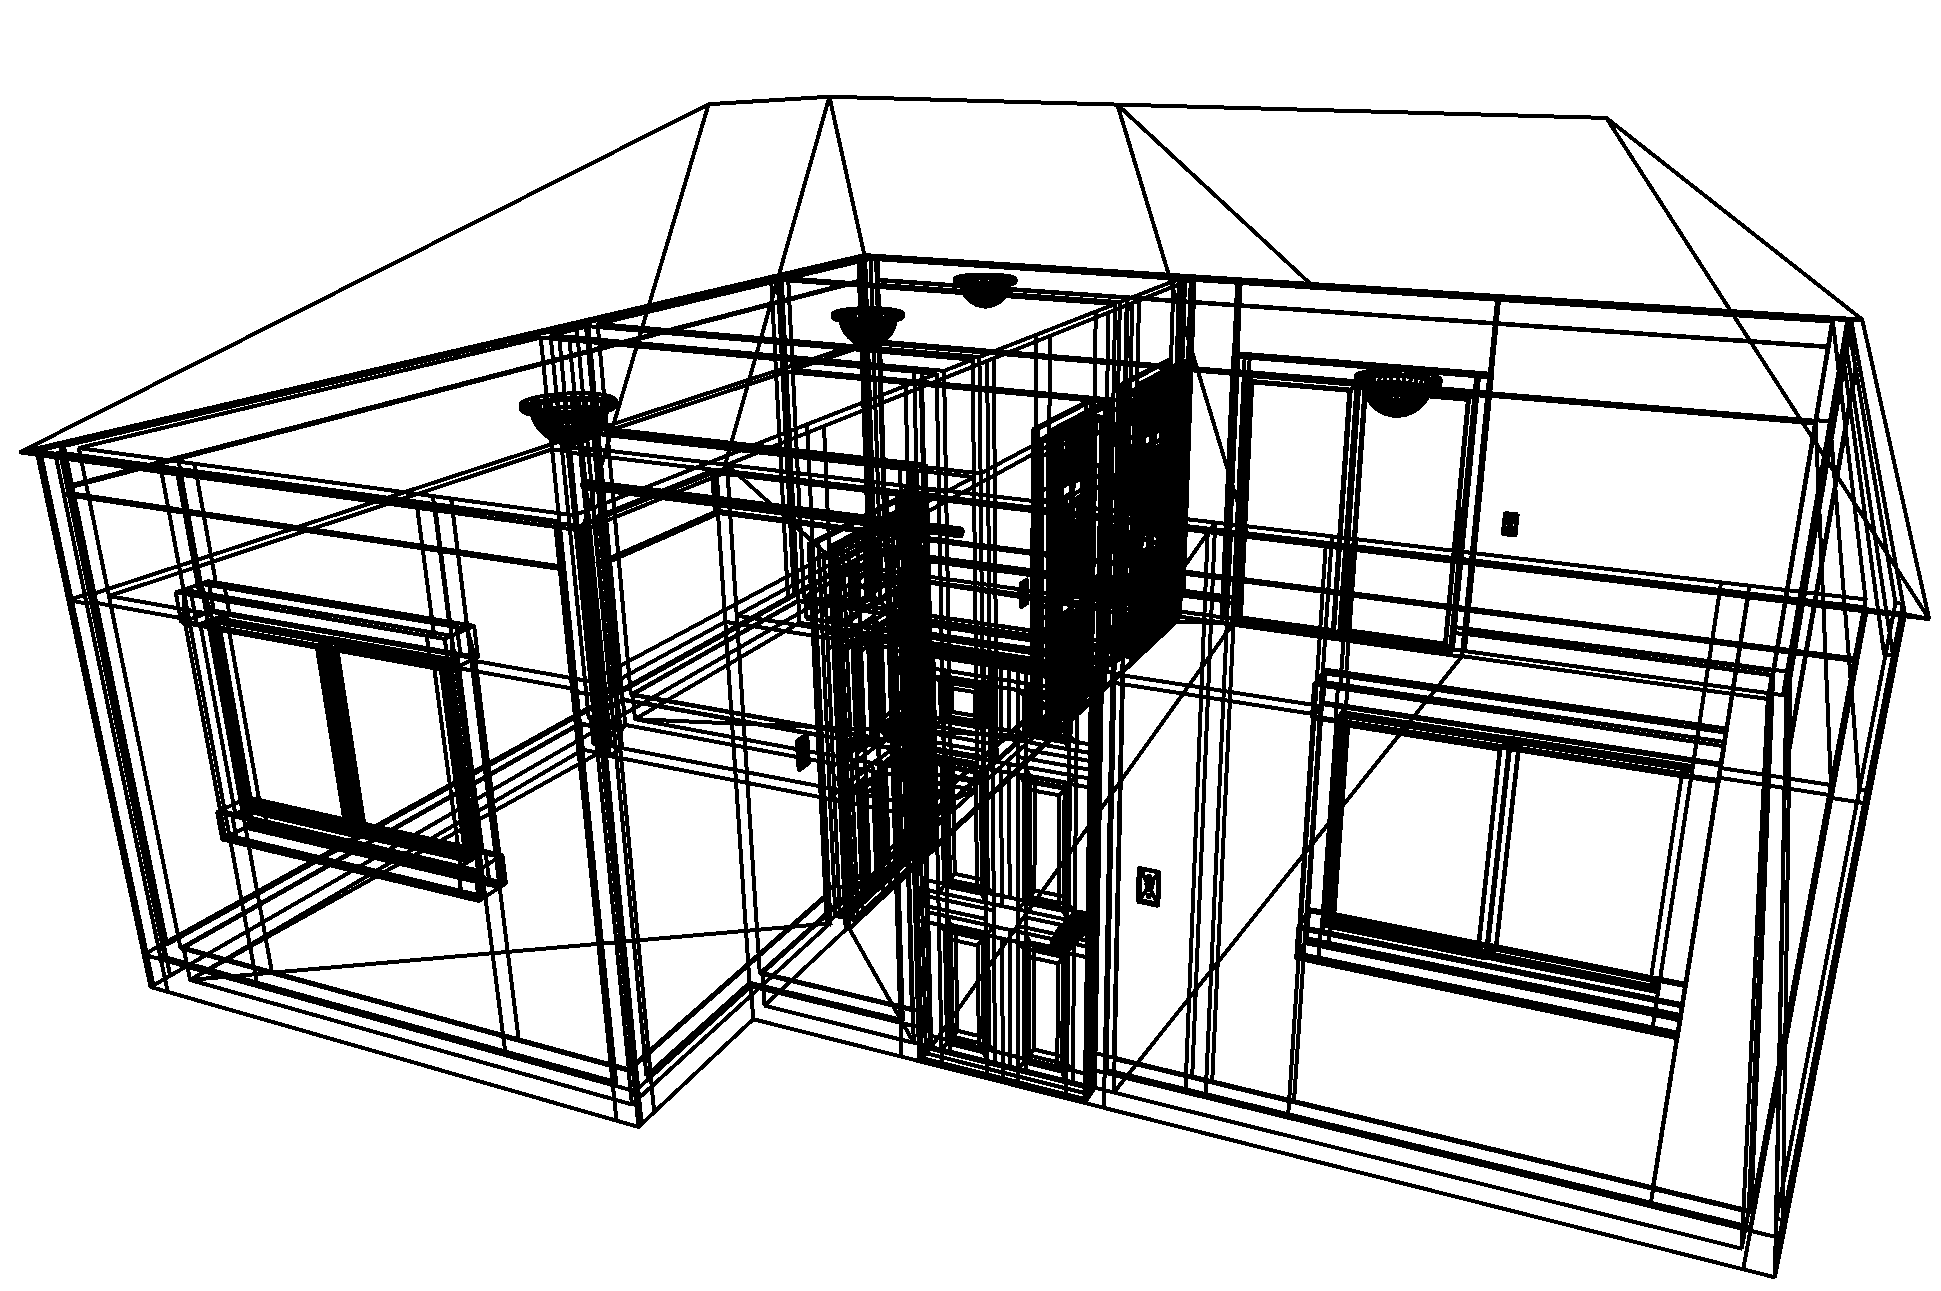
\includegraphics[width=\textwidth]{figures/experiments/house.png}
    \end{center}
    \caption[House with $K=8367$ obstacles]{House with $K=8367$ obstacles}
    \label{fig:house}
\end{figure}


\textbf{Sources $S_i$ and Receivers $R_j$}\newline
Receivers and sources can be specified in CSV files where each line represents the position of a source or a receiver. 
Format is \texttt{"x, y, z"}.
For now only positions are being loaded.

\section{Matryoshka Cube Test}
The purpose of the "Matryoshka Cube" test is to measure the simulation time of the Ray Tracer module with increasing number of objects $K$.
One property of the Matryoshka Cube is that most of paths checked obviously do not exist.
The current strategy ignores certain geometric conditions.
Future strategies can be evaluated with this test and therefore tell if an improvement is measurable or not.
Evaluating \eqref{eq:complex} for $L=3$ and for $K \gg M,N$ it is clear that the problem is of order $O(K^3)$ with the current strategy.

For the Matryoshka Cube Test a single receiver $R_1$ and a single source $S_1$ at position $(0,0,0)$ will be used.
The number of $K$ objects will be doubled in each step and the simulations will run with reflection orders $L=2$ and $L=3$.
In \tabref{tab:matryoshka} you can see the results of that test.

\begin{table}[H]
    \centering
    % spacing in table
    \ra{1.3}
    \begin{tabular}{llll}
      \toprule
      $X$ & $K$ & $L=2$ [s] & $L=3$ [s] \\ \midrule
      1	& 6 & 0.03	& 0.071	         \\
      2	    & 12	& 0.034	& 0.072 	 \\
      4	    & 24	& 0.034	& 0.078	   \\
      8	    & 48	& 0.03	& 0.12	   \\
      16    & 96	& 0.032	& 0.501	   \\
      32    & 192	& 0.042	& 3.268	   \\
      64    & 384	& 0.09	& 25.094	 \\
      128   & 768	& 0.253	& 193.004  \\
      \bottomrule
    \end{tabular}

    \caption[Matryoshka Cube Test Results]{Matryoshka Cube Test Results}
    \label{tab:matryoshka}
\end{table}


First thing to notice is that for second order reflections $L=2$ we still get reasonable run times for $K=768$.
Adding another layer of paths by increasing the allowed reflection order to $L=3$ the weight of the problem becomes clear.
For $K>32$ the factor of $2^3=8$ can be seen in the simulation time.

Nonetheless this was an expected behavior for the chosen strategy and for an increasing number of obstacles and it leaves room for improvement.

\section{Tube Test}
The purpose of the "Tube" test is to measure the simulation time of the Path Sampler module with increasing number of paths and sampling time.
One important property of the Tube is that for every pair $(S_i, R_j)$ which lies between the floor and the ceiling the maximum number of paths exist.
The maximum number of paths is given by \eqref{eq:complex}.
Using this equation and inserting $K=2, L=3$ for the Tube we can get following number of paths for $M$ sources and $N$ receivers:

\begin{equation}
    C_3 = M \cdot N \cdot (1 + 2 \cdot 3) = 7 \cdot M \cdot N
\end{equation}

In \tabref{tab:tube} you can see the results for a single receiver $R_1$ at position $(0,0,0)$ and $M$ sources distributed evenly across the room, between the floor and the ceiling.
It includes runs for different sampling durations $t$.

\begin{table}[H]
    \centering
    % spacing in table
    \ra{1.3}
    \begin{tabular}{lllll}
      \toprule
      $M$ & $C_3$ & $t=0.1 [s]$ & $t=0.3 [s]$ & $t=0.5 [s]$ \\ \midrule
      1 & 7 & 0.008 & 0.010 & 0.016  \\
      8 & 56 & 0.027 & 0.076 & 0.128   \\
      27 & 189 & 0.086 & 0.261 & 0.438   \\
      64 & 448 & 0.203 & 0.618 & 1.034   \\
      125 & 875 & 0.397 & 1.218 & 2.044   \\
      216 & 1512 & 0.695 & 2.132 & 3.571   \\
      343 & 2401 & 1.114 & 3.417 & 5.731   \\
      512 & 3584 & 1.687 & 5.138 & 8.555   \\
      729 & 5103 & 2.394 & 7.309 & 12.235   \\
      1000 & 7000 & 3.286 & 10.284 & 16.933  \\
      \bottomrule
    \end{tabular}

    \caption[Tube Test Results]{Tube Test Results}
    \label{tab:tube}
\end{table}


We can see a linear behavior for increasing number of sources $M$ and increasing sampling time $t$.
This was expected given the complexity relation between sources, receivers and number of objects in \eqref{eq:complex}.

For implementation details check the source code of \texttt{test/TestTube.cpp}.

\section{LOS Estimator}
The LOS (line-of-sight) multilateration estimator shows how ARTS can be used to estimate the location of $M$ sources using $N \geq 4$ receiver nodes in the Reference Room.
The implementation is based on Zhou Yu's paper \cite{zhou2009efficient}.
The main idea of multilateration is to use a predefined set of receivers $R$ and estimate the location to an unknown source $S_i$ by using the travel time from the source to each receiver node.
This of course requires that the source is in line-of-sight of each receiver node.
The minium number of receivers for such a system in 3D space is 4.
More nodes can be added to minimize the error of the estimated location.

In the current implementation $M=1000$ sources are evenly distributed in the Reference Room.
For the LOS localization system the receivers $R = \{ R_1(0,0,0)$, $R_2(1,0,0)$, $R_3(0,1,0)$, $R_4(0,0,1) \}$ will be used.
The simulator will run only for direct paths $L=0$ because reflections are not needed and therefore would be discarded anyway.
By getting the room impulse response (RIR) mentioned in \secref{sec:modelSimplification} the travel time can easily be obtained.

\textbf{Output of the test:}
\begin{verbatim}
# of Paths: 4000
0-Paths: 4000
# of Samples: 400000000
Error avg: 0.000452092
Error min: 0
Error max: 0.00141538
\end{verbatim}

For the evaluation of the estimated locations the euclidean distance has been used.
Since we didn't add any noise to our simulation the error is expected to be very low.
The seen error is due to sampling inaccuracies which is an effect that can not be avoided.
The magnitude of the error is in this particular case negligible.

For implementation details check the source code of \texttt{test/TestLOSEstimator.cpp}.
